\documentclass[10pt,a4paper]{article}
\usepackage[utf8]{inputenc}
\usepackage{amsmath}
\usepackage{amsfonts}
\usepackage{amssymb}
\usepackage{tikz}
\usetikzlibrary{shapes, positioning, decorations.text}
\usepackage{wrapfig}

\begin{document}
\title{Trebuchet}
	\section{Optimum Release Angle}
		At what angle should a projectile be launched to achieve the greatest range?
		If the angle is too large the projectile will go very high but will not have much forward velocity.
		If the angle is too low the projectile will be moving forward very quickly but will not be in the air long enough to make it anywhere.
		What angle will balance these two scenarios and provide the optimum altitude with the best forward velocity?
		Do you have a guess? Think of throwing a ball. What angle do you use when you are trying to really get it to go far?
		Should we use that guess, or can we use our knowledge of math to \emph{prove} what will be the best angle?
		
		\begin{figure}
		\begin{tikzpicture}
			\draw[style=dashed] (0, 0) .. controls (2,3) and (6,3) .. (8, 0);
			\draw[->,ultra thick] (0,0)--(10,0) node[right]{$x$};
			\draw[->,ultra thick] (0,0)--(0,5) node[above]{$y$};
			\node[cross out, draw] at (8,0) {};
			\draw[->, thick] (0,0) -- (2,3) node[midway, above, sloped] (TextNode) {$V$};
			\draw (2,0) arc (0:56:2) node[pos=0.4, above] (TextNode) {\large{$\theta$}};
			\node at (8,-0.4) {$R$};
		\end{tikzpicture}
		\caption{What value of $\theta$ will produce the largest $R$?}
		\label{fig:launchAngle}
		\end{figure}
		
	\subsection{Breakup $V$ into its  X and Y Components}
		The first step is to break up our initial velocity vector $V$ into its two component vectors $V_x$ and $V_y$.
		This will tell us how fast our projectile is moving in these two directions.
		
		\begin{wrapfigure}{l}{0.44\textwidth}
		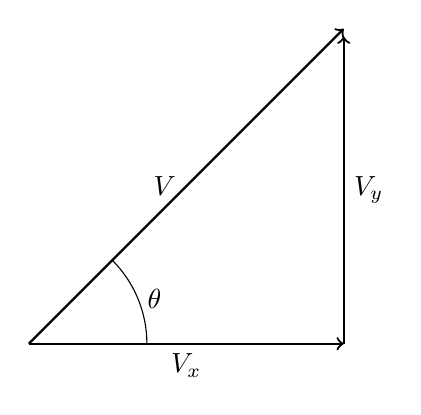
\begin{tikzpicture}
			\draw[->, thick] (0,0)--(4,0) node[below, midway] {$V_x$};
			\draw[->, thick] (4,0)--(4,3.9) node[right, midway] {$V_y$};
			\draw[->, thick] (0,0)--(4,4) node[left, midway] {$V$};
			\draw (1.5,0) arc (0:45:1.5) node[midway, right] {$\theta$};
		\end{tikzpicture}
		\caption{Component Vectors of $V$.}
		\label{fig:componentVectors}
		\end{wrapfigure}
		
		\noindent
		$V =$ launch velocity \\
		$\theta =$ launch angle \\
		$V_x =$ velocity in the $x$ direction \\
		$V_y =$ velocity in the $y$ direction \\
		
		How do we find the values of $V_x$ and $V_y$?
		Since we know that $V_x$ and $V_y$ form a right angle we can use the basic trig identities for $\sin, \cos, \tan$ to find the these values knowing only $V$ and $\theta$.
		Recall from trigonometry the mnemonic SOH-CAH-TOA.
		$V$ is our hypotenuse, H, and based on our $\theta$ location $V_y$ is the opposite, O, and $V_x$ is our adjacent, A.
		\clearpage
		With this information we can form the two equations:
		\[\sin\theta = \frac{V_y}{V} \quad, \quad \cos\theta = \frac{V_x}{V}\]
		Multiplying both sides of each equation by $V$ gives us the component vectors we want.
		\begin{equation}
			V_x = V \sin\theta \quad, \quad V_y = V \cos\theta
			\label{eq:componentVectors}
		\end{equation}
		
	\subsection{Distance Equation}
		Now that we know how fast the projectile is moving in each direction we can figure out far our projectile will travel.
		We know how fast the projectile is moving forward and if we knew how long it had to move forward we would know how far it went.
		The velocity in the y direction is what will determine how long our projectile will be in the air.		
		\begin{equation}
			S = X_i + V_i t + \frac{1}{2}at^2
			\label{eq:posEquation}
		\end{equation}
		where: \\
		$S =$ distance traveled \\
		$X_i =$ initial position \\
		$V_i = $ initial velocity \\
		$a =$ acceleration \\
		$t =$ time \\
		With this equation we can determine the position of our projectile in any one direction at any time.
		Since we need to know how long the projectile will be in the air we will work with $V_y$ first.
	\subsubsection{Flight Time}
		To determine how long the projectile will be in the air we can use just the $V_y$ component of our velocity vector and ignore $V_x$.
		We will assume that our projectile starts at $y=0$.
		It will be an exercise for the reader to determine if a higher starting height changes the optimum launch angle.
		We want to know the time, $t$, at which a projectile will return back to the ground after starting straight up at our initial velocity in y.
		Substituting in our known values we get the formula:
		\[\underbrace{0		\rule[-3pt]{0pt}{5pt}}_{\mbox{end pos}}
		  = \underbrace{0 		\rule[-3pt]{0pt}{5pt}}_{\mbox{initial pos}}
		  + \underbrace{V_yt	\rule[-3pt]{0pt}{5pt}}_{\mbox{$V\sin(\theta)t$}}
		  + \frac{1}{2}
		  \underbrace{-9.8		\rule[-3pt]{0pt}{5pt}}_{\mbox{gravity $m/s^2$}}
		  t^2  \]
		This provides us with a quadratic equation which contains just one unknown value $t$.
		For equations with the form:
		\begin{equation}
			ax^2 + bx + c = 0
		\end{equation}
		we can use the quadratic formula to solve for $x$.
		The quadratic formula is:
		\begin{equation}
			x = \frac{-b \pm \sqrt{b^2 - 4ac} }{2a}
			\label{eq:quadraticFormula}
		\end{equation}
		
		
		 
		
\end{document}